
	\section{Resultados}
	Esta sessão apresenta e analisa os resultados obtidos com a realização de testes descritos anteriormente.
	\\
	
	\subsubsection{Teste de latência}
	Primeiramente descreve o resultado do processo de leitura para teste de latência.
	Como no gráfico da Figura~\ref{fig:latencia_l} é difícil distinguir as linhas de cada RAID por ter valores de latência bem próximos entre eles, foi colocado a Tabela~\ref{tab:latencia_l} para mostrar a diferença dos valores.
	Os resultados representam a média dos 1000 operações, descartando-se 10\% dos com maior desvio.
	 \\
	 
	De acordo com Tabela~\ref{tab:latencia_l} o RAID 1 apresenta menor valor de latência entre todos os tipos de RAID quando o arquivo tem tamanho de 1KB ou 100KB. Contudo, quando os arquivos crescem de tamanho, ficando com 1MB e 10MB, o resultado reverte deixando o RAID 1 com a latência mais alta de todos. 
	Isso pode ser explicado pelo fato de que nos RAID 0 e RAID 5 ocorrem a reconstrução de arquivo a partir de alguns pedaços de dados, cujo este procedimento extra possui maior custo de tempo que a transmissão de dados quando trata de arquivos pequenos. Porém, o custo entre dois se aproxima conforme aumenta o tamanho do arquivo e a sua relação inverte quando ultrapassa de um determinado tamanho.
	%Olhando no gráfico da Figura~\ref{fig:latencia_l} esta inversão ocorre aproximadamente no ponto intermediário entre tamanhos de 100KB e 1MB, tanto para RAID 0 quanto para RAID 5, dando um valor aproximado de 500KB.
	\\
	
	Também existe o fato de que no RAID 1 ocorre simples espelhamento de dados, significando que para obter o arquivo basta comunicar com um dos servidores, enquanto nos outros dois tipos de RAID os clientes sempre necessitam se comunicar com múltiplos servidores para realizar a mesma operação. Por isso, o RAID 1 tem possibilidade de concluir a operação de forma mais rápida que RAID 0 e RAID 5. Porém, como a conexão entre cliente e os servidores de armazenamento foi implementado em forma de \textit{multithread}, aparentemente as transmissões que ocorrem entre eles acontecem simultaneamente quando realiza uma operação. Por isso, supormos que a sua influência pode não ser muito grande suficiente a ponto de mudar o resultado do teste.
	\\
	
	Assim, pelos fatos acima apresentados e pelos valores da Tabela~\ref{tab:latencia_l}, é possível considerar que no processo de leitura do arquivo a latência para cada tipo de RAID tem relação de RAID 0 < RAID 5 < RAID 1, sendo como exceção quando trata de arquivos menores.
	\\
	
	\begin{figure}[h]
		\begin{tabular}{lc}
			\begin{minipage}{.50\textwidth}
				\begin{center}
					
					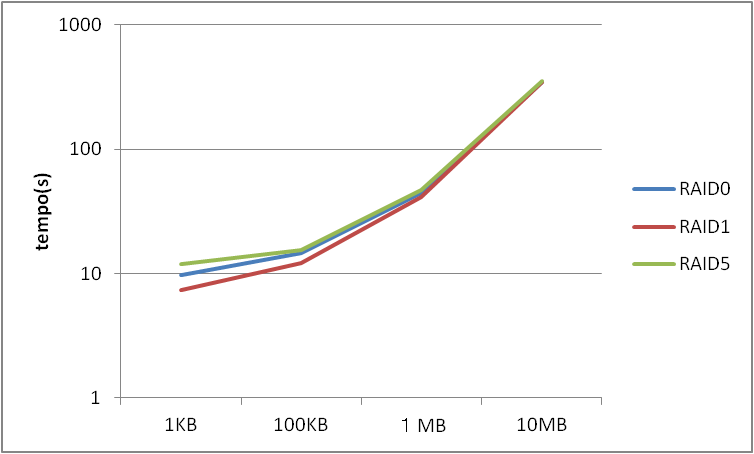
\includegraphics[clip,width=8.0cm]{images/resultados/latencia_leitura.png}
					\caption{Gráfico de latência pata leitura}
					\label{fig:latencia_l}
					
				\end{center}
				
			\end{minipage}
			
			\begin{minipage}{.5\textwidth}
				\makeatletter
				\def\@captype{table}
				\makeatother
				\caption{Tabela de latência pata leitura(s)}
				\label{tab:latencia_l}
				\begin{center}
					\begin{tabular}{|c|c|c|c|c|} \hline
								& 1KB  & 100KB & 1MB   & 10MB  \\ \hline
						RAID 0	& 9.33 & 12.26 & 38.84 & 324.73\\ \hline
						RAID 1	& 9.01 & 12.19 & 41.50 & 348.15\\ \hline
						RAID 5	& 9.76 & 12.62 & 40.11 & 326.75\\ \hline
						
						
					\end{tabular}
				\end{center}
				
			\end{minipage}
		\end{tabular}
	\end{figure}
	
	
	%A Figura~\ref{fig:latencia_e} mostra o gráfico e a Tabela~\ref{tab:latencia_e} mostra a tabela de resultado do teste para escrita de arquivos.
	
	No caso de teste para escrita de arquivo a diferença dos valores da latência para cada tipo de RAID ficou bem nítida comparado com resultado obtido na operação de leitura, como mostram a Figura~\ref{fig:latencia_e} e a Tabela~\ref{tab:latencia_e}.
	\\
	
	De acordo com o gráfico da Figura~\ref{fig:latencia_e}, o crescimento da linha de RAID 1 é mais intensa de todos, onde é esperado que a diferença comparado com outros tipos de RAID tende a aumentar cada vez que o tamanho de arquivo cresce.
	\\
	
	No gráfico aparentemente o RAID 1 possui a maior latência de todos para qualquer tamanho do arquivo. Contudo, olhando na Tabela~\ref{tab:latencia_e} percebe-se que para os arquivos de 1KB e 100KB o RAID 5 apresenta maior latência do que o RAID 1. Isto pode ser explicado com a mesma razão que ocorreu em teste para leitura, onde se o tamanho do arquivo é pequeno o tempo para dividir o arquivo em pedaços de dados é mais demorado que o tempo para enviar estes dados. Aproximadamente a partir de 100KB, a latência do RAID 1 supera o valor dos RAID 0 e RAID 5, de acordo com gráfico. 
	\\
	%Também pode ser citado que no RAID 5 existe uma etapa extra de criar o bloco de paridade e que 
	
	Mesmo para operação de escrita a latência mantém relação de RAID 0 < RAID 5 < RAID 1 para maioria dos casos, ou seja, quando trata de arquivos com tamanhos maiores que 100KB.
	\\
	
	\begin{figure}[h]
		\begin{tabular}{lc}
			\begin{minipage}{.50\textwidth}
				\begin{center}
					
					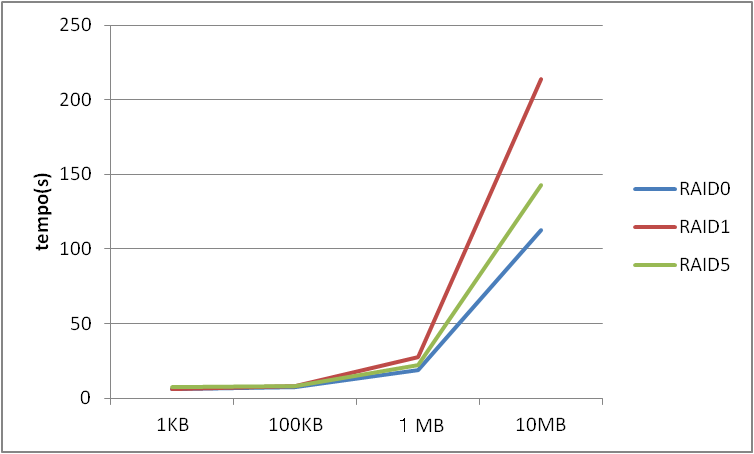
\includegraphics[clip,width=8.0cm]{images/resultados/latencia_escrita.png}
					\caption{Gráfico de latência pata escrita}
					\label{fig:latencia_e}
					
				\end{center}
				
			\end{minipage}
			
			\begin{minipage}{.5\textwidth}
				\makeatletter
				\def\@captype{table}
				\makeatother
				\caption{Tabela de latência pata escrita(s)}
				\label{tab:latencia_e}
				\begin{center}
					\begin{tabular}{|c|c|c|c|c|} \hline
								& 1KB  & 100KB & 1MB   & 10MB \\ \hline
						RAID 0	& 6.70 & 6.91 & 14.92 & 101.93\\ \hline
						RAID 1	& 6.79 & 7.53 & 23.79 & 213.94\\ \hline
						RAID 5	& 7.31 & 7.91 & 18.26 & 134.31\\ \hline
						
					\end{tabular}
					
				\end{center}
			\end{minipage}
		\end{tabular}
	\end{figure}
	
	\subsubsection{Teste de vazão}
	Agora apresentamos a descrição do resultado obtido no teste de vazão, para operação de leitura de arquivo. O gráfico e os valores são mostrados respectivamente nas Figura~\ref{fig:throughput_l} e Tabela~\ref{tab:throughput_l}.
	\\
	
	Neste resultado também o RAID 1 mostrou o comportamento já visto no teste de latência, onde os arquivos de tamanhos de 1KB e de 100KB possuírem maiores valores de vazão de todos, enquanto tamanhos de 1MB e 10MB apresentam menores valores de todos. A explicação para este fato pode ser a mesma que foi analisado no teste anterior, o que considera a relação de custo de tempo entre o processo de reconstrução e a transmissão de dados.
	\\
	
	No gráfico da Figura~\ref{fig:throughput_l} podemos observar que a linha de RAID 0 supera a linha de RAID 1 no ponto aproximado de 250KB, enquanto a linha de  RAID 5 somente consegue superar no ponto aproximado de 500KB. 
	Esta diferença relativamente grande de tamanho para superar a linha do RAID 1 não foi observado no teste de latência, apresentando tamanhos bem próximos entre RAID 0 e RAID 5. Este fato pode ser explicado por existência de vários clientes em operação ao mesmo tempo, diferentemente do teste de latência que existia um único cliente, cujo a pequena diferença do custo de tempo entre RAID 0 e RAID 5 não foi explícita.
	\\
	
	Depois que o tamanho do arquivo passa de 1MB, as linhas da taxa de vazão dos três tipos de RAID começam a se aproximar, aparentemente convergindo em um único valor no ponto de 10MB. Porém, pela Tabela~\ref{tab:throughput_l} é possível observar que a relação das taxas ainda continuam RAID 0 < RAID 5 < RAID 1.
	\\
	
	Em geral, exceto quando trata de arquivos maiores que 500KB, podemos considerar que a taxa de vazão para leitura de arquivo entre três tipos de RAID obedecem a relação de RAID 0 > RAID 5 > RAID 1, como esperado.
	\\
	
	\begin{figure}[h]
		\begin{tabular}{lc}
			\begin{minipage}{.50\textwidth}
				\begin{center}
					
					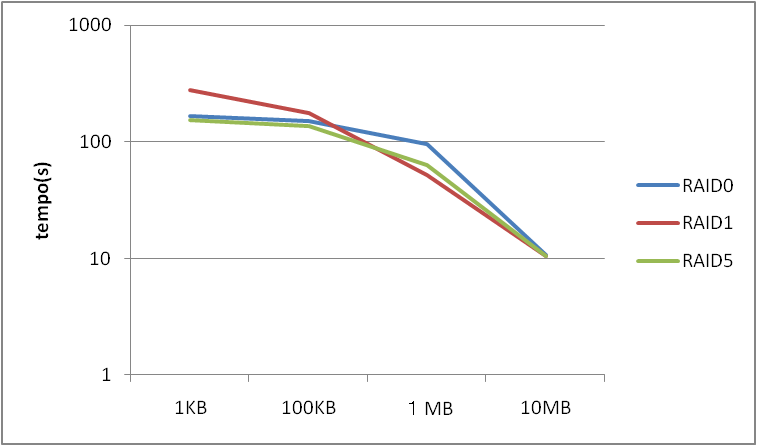
\includegraphics[clip,width=8.0cm]{images/resultados/throughput_leitura.png}
					\caption{Gráfico de vazão para leitura(ops/s)}
					\label{fig:throughput_l}
					
				\end{center}
				
			\end{minipage}
			
			\begin{minipage}{.5\textwidth}
				\makeatletter
				\def\@captype{table}
				\makeatother
				\caption{Tabela de vazão para leitura}
				\label{tab:throughput_l}
				\begin{center}
					\begin{tabular}{|c|c|c|c|c|} \hline
						& 1KB & 100KB & 1MB & 10MB \\ \hline
						
						RAID 0	& 167.14 & 151.63 & 95.08 & 10.63\\ \hline
						RAID 1	& 278.86 & 177.43 & 51.92 & 10.52\\ \hline
						RAID 5	& 152.79 & 135.30 & 63.34 & 10.56\\ \hline
						
					\end{tabular}
				\end{center}
				
			\end{minipage}
		\end{tabular}
	\end{figure}
	
	
	O último experimento feito é o teste de vazão para escrita de arquivos.
	Diferentemente dos resultados obtidos pelos testes anteriores, em que o RAID 1 apresentava melhor desempenho para casos de arquivos pequenos, o gráfico da Figura~\ref{fig:throughput_e} mostra que o RAID 0 apresenta o melhor valor para a taxa de vazão independentemente de tamanho do arquivo. 
	Contudo, observando a inclinação das linhas de RAID 0 e RAID 1, supomos que a inversão do custo de tempo entre a divisão de arquivo e o envio de dado já acontecem em algum tamanho menor que 1KB. Assim, podemos considerar que este gráfico também apresenta o mesmo comportamento visto nos testes anteriores. 
	\\
	Em tamanho aproximado de 25KB a linha de RAID 5 ultrapassa a linha de RAID 1 e depois que o tamanho do arquivo chega em 100KB, todas as linhas de RAID começam a prosseguir de forma quase paralela entre si.
	\\
	
	Assim, quando consideramos arquivo de tamanhos maiores que 25KB, a taxa de vazão entre os três tipos de RAID possui relação de RAID 0 > RAID 5 > RAID 1.
	\\
	
	\begin{figure}[h]
		\begin{tabular}{lc}
			\begin{minipage}{.50\textwidth}
				\begin{center}
					
					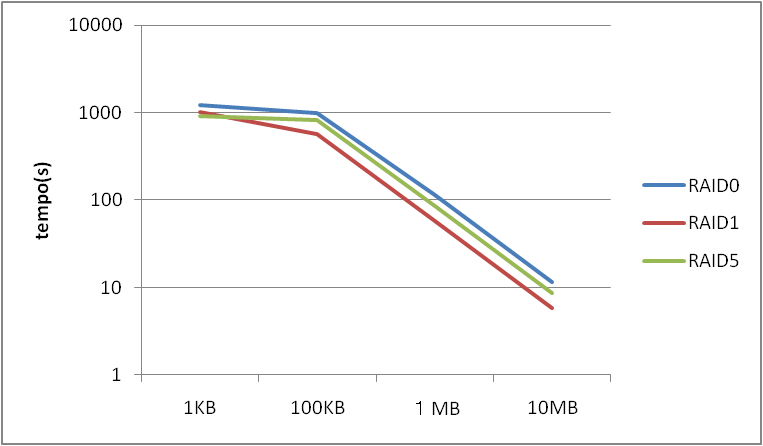
\includegraphics[clip,width=8.0cm]{images/resultados/throughput_escrita.png}
					\caption{Gráfico de vazão para escrita}
					\label{fig:throughput_e}
					
				\end{center}
				
			\end{minipage}
			
			\begin{minipage}{.5\textwidth}
				\makeatletter
				\def\@captype{table}
				\makeatother
				\caption{Tabela de vazão para escrita}
				\label{tab:throughput_e}
				\begin{center}
					\begin{tabular}{|c|c|c|c|c|} \hline
						& 1KB & 100KB & 1MB & 10MB \\ \hline
						
						RAID 0	& 1209.19 & 988.14 & 113.07 & 11.51\\ \hline
						RAID 1	& 1023.54 & 571.43 & 58.01  & 5.76 \\ \hline
						RAID 5	& 914.91  & 830.56 & 84.52  & 8.66 \\ \hline
						
						
					\end{tabular}
				\end{center}
				
			\end{minipage}
		\end{tabular}
	\end{figure}
	
	\section{Conclusões do Capítulo}
	
	Depois de obter os resultados dos testes, foi possível verificar que o desempenho para leitura e escrita de dados entre os três tipos de RAID possui a relação de RAID 0 > RAID 5 > RAID 1 na maioria dos casos. Observando que 500KB foi o maior tamanho aproximado em que ocorre a inversão da relação de custo de tempo entre a transmissão de dados e o processo de divisão ou reconstrução de arquivo, quando trata de arquivos com tamanho desta ordem a vantagem que RAID 1 tem sobre RAID 5 pode ser considerado bem pequena. 
	Por exemplo, na latência para leitura de arquivo de 100KB o RAID 1 ganha do RAID 5 somente por 0,43 segundos, enquanto para arquivo de 1MB o RAID 5 é 1,39 segundos mais vantajoso que o RAID 1.
	\\
	
	Assim, podemos dizer que o RAID 5 conseguiu cobrir as desvantagens que existem nos RAID 0 e RAID 1, conseguindo ter a segurança nos arquivos armazenados sem perder muito o desempenho para a transmissão e o armazenamento.
	\\
	
	
	
	
	
	
	
	
	
	
	
	
	